Diversos trabalhos têm surgido na academia propondo aplicações práticas de computação ubíqua. No entanto, cada domínio de aplicação possui suas peculiaridades e apresenta seu modelo de falhas característico. Esta seção destina-se a apresentar estudos de caso da academia onde soluções gerais e específicas são empregadas no sentido de tolerar falhas nestes sistemas.

\subsection{CoBrA} % (fold)
\label{sub:cobra}

CoBrA (\emph{\textbf{C}ontext \textbf{Br}oker \textbf{A}rchiecture}) é um \emph{middleware} de computação ubíqua que fornece serviços básicos para a aquisição e gerenciamento de informação contextual em espaços inteligentes (\emph{smart spaces}). O objetivo de CoBrA é permitir que agentes distribuídos em um ambiente ubíquo possam acessar um modelo compartilhado de contextos, contribuir com informações para este modelo e gerenciar o acesso de terceiros a suas informações contextuais em um ambiente ubíquo com sensibilidade o contexto.

CoBrA possui uma arquitetura \emph{broker-centric}, ou seja, existe um agente central (\emph{broker}) que faz inferências sobre as informações contextuais dos demais agentes do ambiente e serve como intermediário de todas as trocas de informações contextuais entre os demais agentes. Podemos ainda ter redes de \emph{brokers} trocando informações contextuais sobre os agentes presentes em seus respectivos espaços inteligentes, como é o caso do sistema ubíquo EasyMeeting~\cite{finin2005semantic}, ilustrado na Figura~\ref{fig:_cobra_easy_meeting}, sistema este construído sobre o CoBrA.

\begin{figure}[htbp]
	\centering
		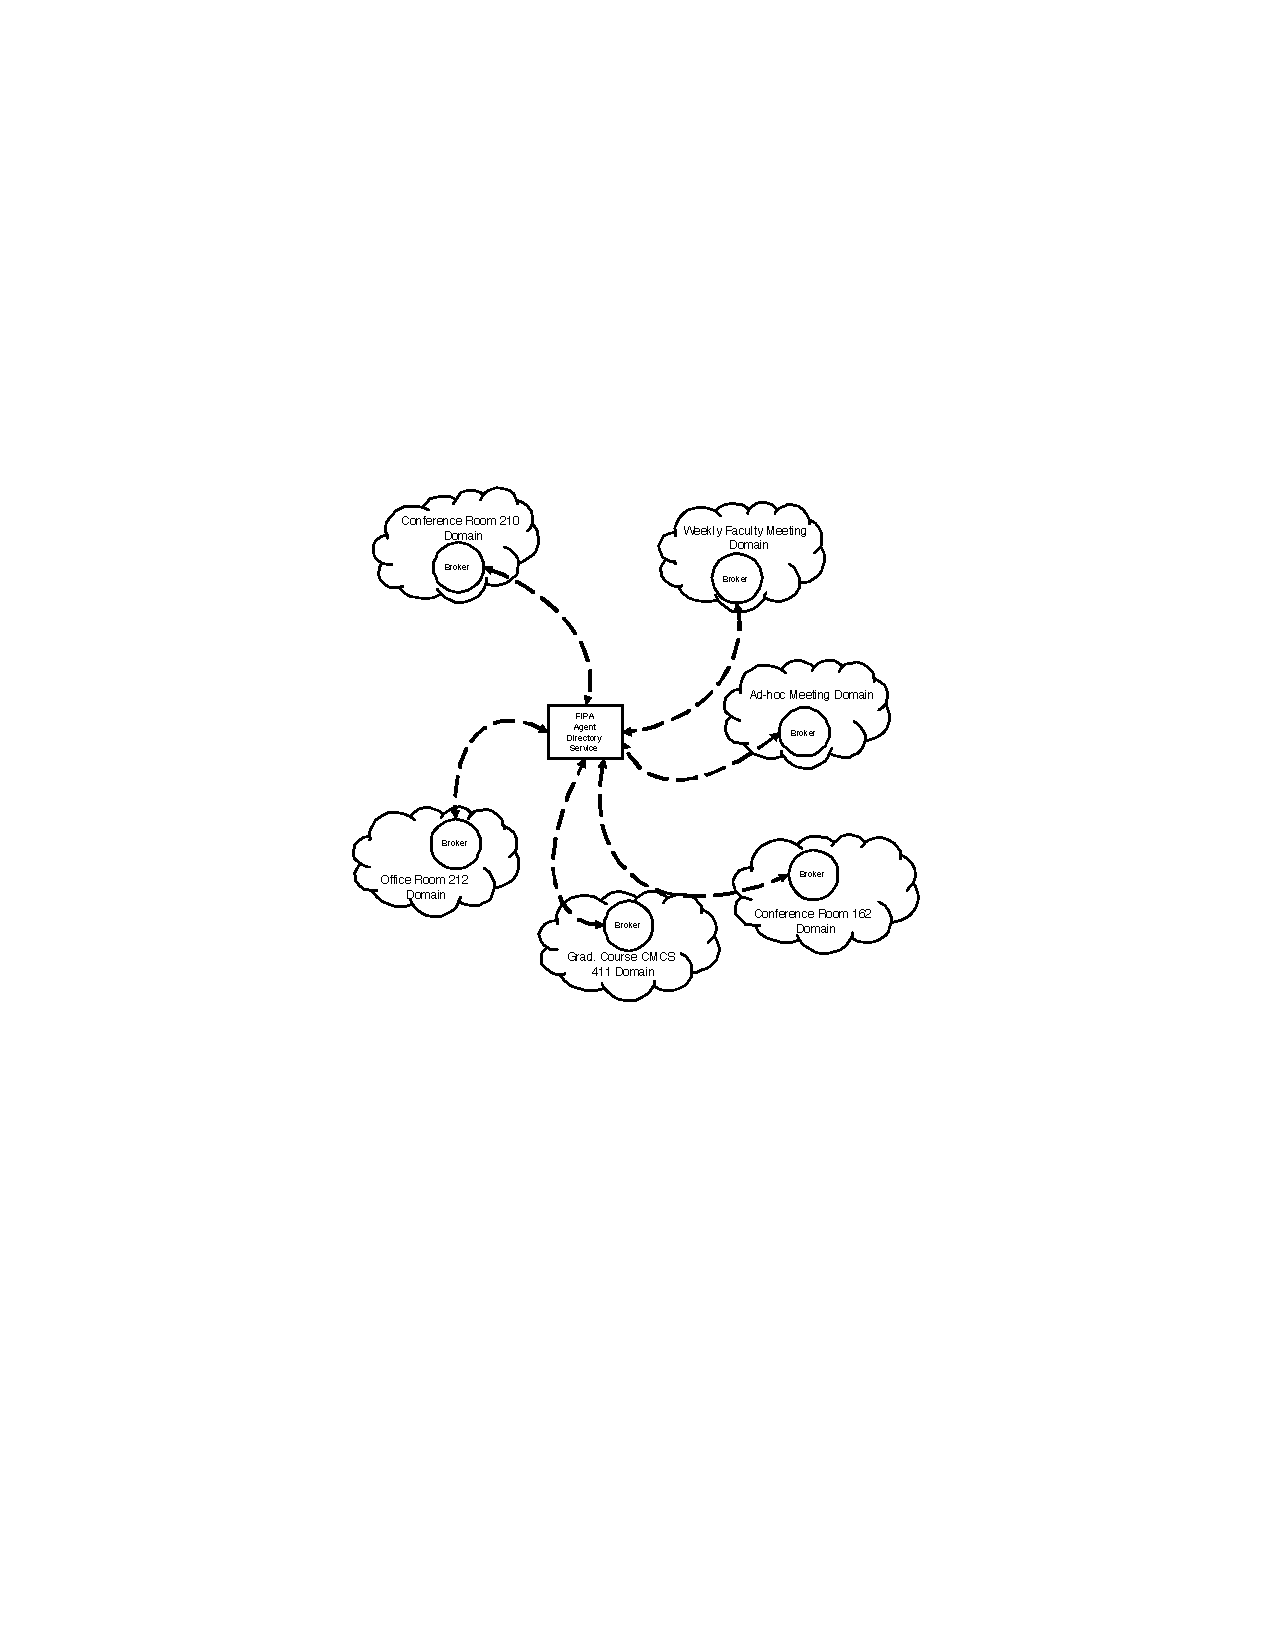
\includegraphics[width=.7\textwidth]{figuras/cobra_easy_meeting.pdf}
	\caption{EasyMeeting: estudo de caso desenvolvido sobre CoBrA.}
	\label{fig:_cobra_easy_meeting}
\end{figure}

CoBrA propõe mecanismos de tolerância a falhas baseados na arquitetura proposta em~\cite{kumar2000adaptive} sobre \emph{times persistentes de brokers}. Tal arquitetura proposta (\emph{Adaptive Agent Architecture}) assume que para um \emph{broker} ingressar em um time, este deve assumir comprometimentos em relação aos serviços que devem prestar, o que facilita a substituição de um \emph{broker} que apresenta falhas e faz com que o sistema forneça funcionalidades básicas enquanto houver pelo menos um \emph{broker} funcionando. Outros comprometimentos que os \emph{brokers} podem assumir lhes dão a permissão para criar/escolher novos \emph{brokers} e incluí-los no time, fazendo com que o sistema consiga se adaptar automaticamente perante variações no ambiente, tais como falhas nos agentes. 

A teoria que embasa estes mecanismos é a \textbf{teoria das intenções conjuntas} (\emph{theory of joint intentions}), amplamente utilizada em ramos da computação ligados à Inteligência Artificial. Este conjunto de técnicas espera, intuitivamente, que um time será mais robusto do que um conjunto de indivíduos. A premissa básica é de que um time trabalha junto para atingir uma determinada meta (por exemplo, prover serviços de contexto). Quando um membro do time está com problemas outros membros do time o ajudarão (por exemplo, um servidor pode ordenar o reinício de um outro servidor que apresenta uma falha transiente e restaurar seu estado) e quando um membro ficar indisponível o restante dos membros farão seu trabalho para cumprir as metas do time (por exemplo, chamadas ao servidor indiponível podem ser atendidas por um outro servidor qualquer do time). Um time deixará de cumprir uma meta global se, e somente se, todos os membros escolherem esta opção. Logo, times são organizações inerentemente tolerantes a falhas.

Em~\cite{kumar2000adaptive} são detalhadas estratégias necessárias para implementar os mecaninsmos de times em software, inclusive os protocolos de comunicação que devem ser usados para a autocoordenação dos times de \emph{brokers}.

% subsection cobra (end)

\subsection{Coda FS} % (fold)
\label{sub:coda_fs}

O Coda File System~\cite{satyanarayanan1990coda} é um sistema de arquivos distribuído descendente do Andrew File System (AFS)~\cite{howard1988overview} e fornece diversos recursos semelhantes aos do AFS. Coda foi projetado para ser um sistema de arquivos escalável, seguro e altamente disponível, com alto grau de transparência de distribuição. Tomando também em consideração a alta disponibilidade, os projetistas do Coda tentaram chegar a um alto grau de transparência na recuperação de falhas. Para obter algum grau de transparência de recuperação de falhas os desenvlovedores do Coda criaram vários mecanismos sofisticados baseados em cache de dados no lado do cliente e replicação de servidores de arquivos.

\subsubsection*{Operação desconectada}

Os clientes Coda, ao contrário de clientes NFS, por exemplo, continuam a operar normalmente mesmo sem conseguir conectar nenhum dos servidores~\cite{kistler1992disconnected}. Uma vez que o cliente abre um arquivo do servidor, este  passa a editar uma cópia local, de forma que, quando o usuário terminar sua sessão sem conexão, não resultará em erro algum. Quando as alterações forem atualizadas no(s) servidor(es), no entanto, pode ser que ocorra algum conflito, o qual nem sempre é resolvido automaticamente. Porém raramente os usuários compartilham um arquivo para escrita, tornando esta situação uma exceção.

Para que a operação desconectada realmente funcione, todos os arquivos que o cliente precisa devem estar em cache. Coda provê um mecanismo sofisticado chamado \emph{hoarding} para garantir isso. O mecanismo funciona como segue. Primeiro, um usuário pode criar uma lista dos arquivos que o mesmo julga serem os mais importantes para ele (\emph{hoard database}). O Coda usa esta lista fornecida pelo usuário juntamente com a localidade de referência aos arquivos para atribuir prioridades a estes. Uma vez que foram atribuídas prioridades a todos os arquivos do usuário, o Coda se vale de três regras básicas para gerenciar a cache:

\begin{enumerate}
	\item Não existe nenhum arquivo fora da cache com prioridade maior que a de um que está na cache;
	\item Ou a cache está cheia ou nenhum arquivo fora da cache tem prioridade não-zero;
	\item Cada arquivo em cache é somente uma cópia de um arquivo no servidor.
\end{enumerate}

Para o Coda, se a cache satisfaz estas 3 regras ela está em estado de \emph{equilibrium}. Contudo as prioridades podem ser alteradas dinamicamente. Para reestabelecer o \emph{equilibrium} da cache, a cada 10 minutos o módulo cliente realiza o que os autores chamam de \emph{hoard walk}, reajustando prioridades e substituindo arquivos na cache. Contudo, embora estas técnicas tenham aumentado muito a eficiência do Coda FS, elas não garantem que todos os dados que o cliente precisará futuramente estarão armazenados em cache no caso de uma operação desconectada.

\subsubsection*{Memória Virtual Recuperável}
Além de prover alta disponibilidade com as operações desconectadas, Coda emprega um mecanismo que facilita a recuperação de um processo em falha. Memória Virtual Recuperável (\emph{Recoverable Virtual Memory} -- RVM) é um mecanismo que armazena estruturas de dados cruciais da a aplicação para uma recuperação rápida em caso de falha (mais detalhes em~\cite{satyanarayanan1994lightweight}).

A ideia do RVM é bastante simples. As estruturas de dados mais importantes da aplicação são mantidas em um espaço conhecido da memória principal e são armazenados logs para cada alteração nestes dados, de maneira semelhante a um esquema de transações, porém sem suporte a concorrência. Em caso de falha de um processo, os dados são restaurados de maneira relativamente fácil através do log de operações nas estruturas de dados mais importantes.

O Coda FS ainda implementa diversos mecanismos de segurança que aumentam ainda mais a confiabilidade dos usuários neste sistema de arquivo.

% subsection coda_fs (end)

\subsection{Prism-MW} % (fold)
\label{sub:prism_mw}

Prism-MW~\cite{Seo07} é uma plataforma de \emph{middleware} que oferece um conjunto de blocos básicos para a construção de sistemas ubíquos. O Prism-MW fornece mecanismos de tolerância a falhas embutidos, ao mesmo tempo que sua arquitetura é eficiente e clara. O \emph{middleware} arquitetural é, basicamente composto por 3 camadas. Na base uma Máquina Virtual, que permite a implantação do sistema em plataformas hetereogêneas sem modificações na implementação. Acima da máquina virtual são fornecidos os blocos básicos de construção da arquitetura (componentes, conectores, eventos, etc.). No topo, usando os componentes da camada arquitetural, são implementados três serviços considerados essenciais para sistemas ubíquos: $(1)$ descoberta dinâmica de novos serviços e recursos, $(2)$ recuperação automática e transparente de falhas e $(3)$ determinação analítica das estratégias de replicação de componentes e arquiteturas de implantação.

\begin{figure}[htbp]
	\centering
		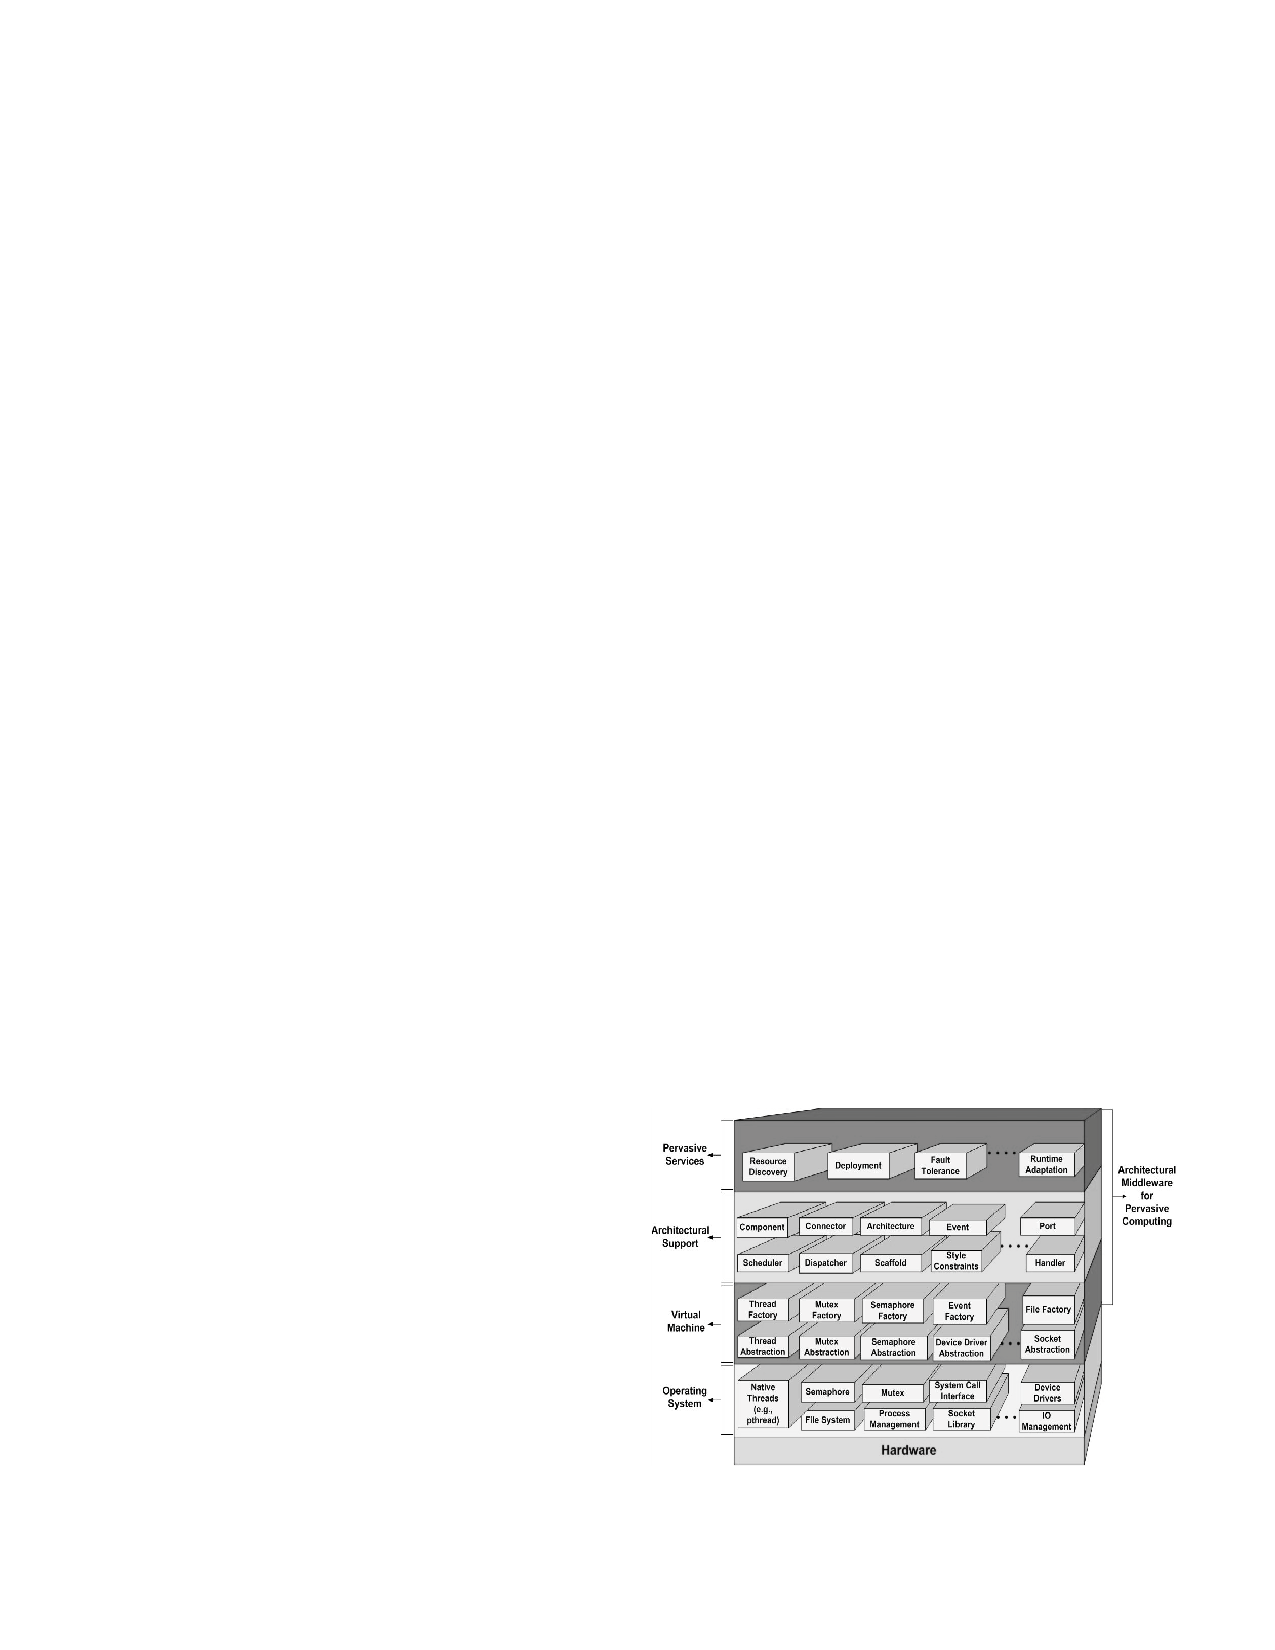
\includegraphics[width=.7\textwidth]{figuras/prism.pdf}
	\caption{Visão geral do \emph{middleware} Prism.}
	\label{fig:prism}
\end{figure}

Como pode ser visto na Figura~\ref{fig:prism} a abordagem do Prism-MW consiste em separar totalmente a lógica da aplicação da lógica de tolerância a falhas, fornecendo esta última como um serviço da camada superior da arquitetura. Esta abordagem consiste basicamente em fornecer \textbf{conectores lógicos} entre os componentes, que oferecem diferentes garantias para os diferentes elementos que irão conectar-se através deles, e módulos que auxiliam no \textbf{gerenciamento de componentes replicados}. A abordagem de Prism auxilia na tarefa de construção, análise e adaptação de software ubíquo mantendo a qualidade de serviço (QoS) em diversos cenários ubíquos~\cite{Seo07}.

% subsection prism_mw (end)

% \subsection{ADRF} % (fold)
% 
% \emph{Assured Dynamic Reconfiguration Framework} (ADRF) é um \emph{framework} qua fornece recursos básicos para a completa e correta reconfiguração de um sistema ubíquo. 

% subsection adrf (end)

% \subsection{GaiaOS} % (fold)
% \label{sub:gaiaos}
% 
% O projeto Gaia consiste de uma plataforma semelhante a um sistema operacional para ambientes ubíquos, que fornece um mecanismo de abstração do acesso aos recursos físicos presentes em um espaço inteligente. Diversos conceitos presentes em sistemas operacionais modernos, como eventos, sinais, sistemas de arquivos e processos, são traduzidos no GaiaOS para o contexto da computação ubíqua. A Figura~\ref{fig:figuras_gaiaos} fornece uma visão geral dos componentes em um sistema GaiaOS. Como pode-se observar nesta ilustração, o \emph{Unified Object Bus} é a espinha dorsal do GaiaOS, pois é o barramento pelo qual todos os dispositivos em um espaço inteligente podem se intercomuncar por uma única linguagem.
% 
% \begin{figure}[htbp]
% 	\centering
% 		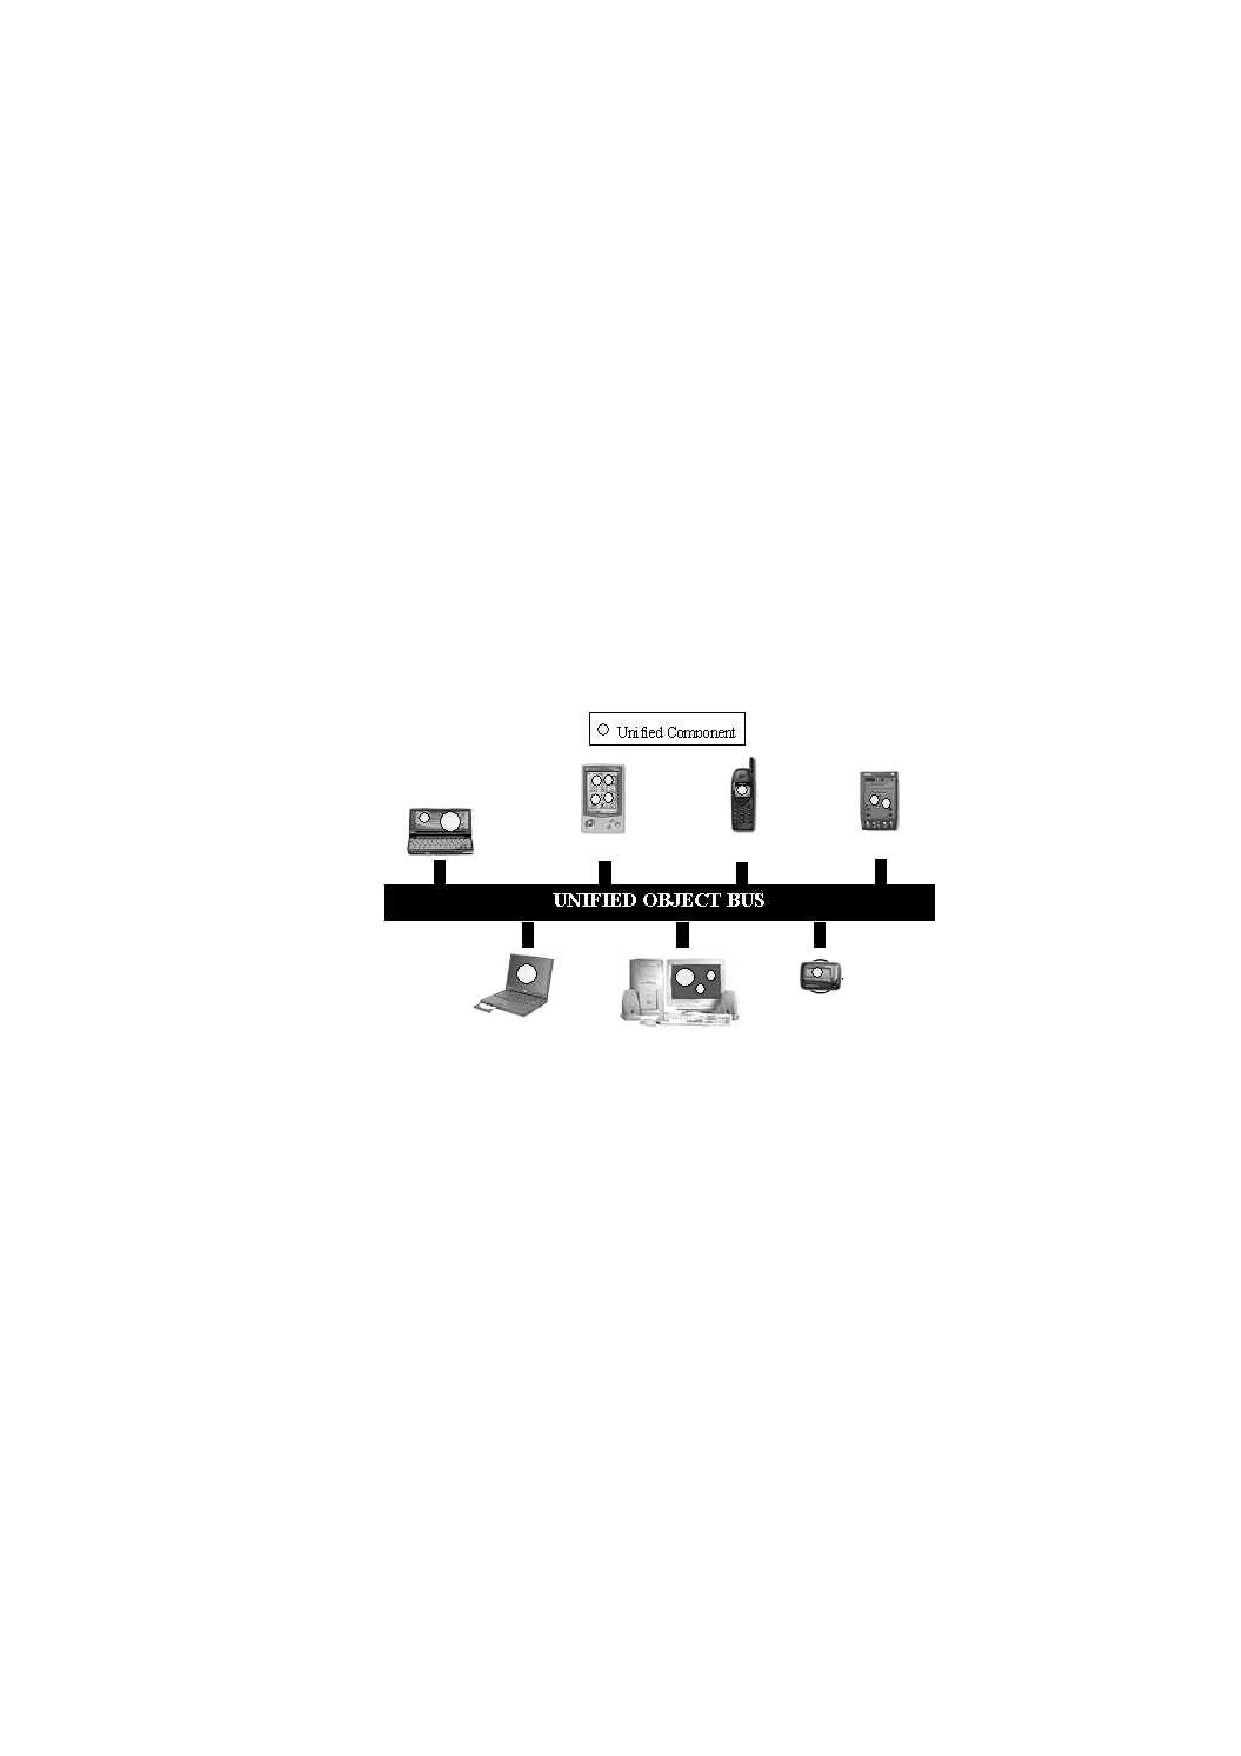
\includegraphics[width=.7\textwidth]{figuras/gaiaos.pdf}
% 	\caption{Visão geral do GaiaOS.}
% 	\label{fig:figuras_gaiaos}
% \end{figure}
% 
% No \emph{kernel} do GaiaOS são implementados serviços de inicialização básica do sistema: gerenciador de eventos; localizador de serviçoos e indivíduos; base de registros de dispositivos; serviços, indivíduos e aplicações ativos no sistema; sistema de arquivos; e serviços de autentitcaçãoo e autorização de usuários.
% 
% A extensão \emph{Gaia Context Infrastructure}~\cite{ranganathan2003middleware} adiciona sensibilidade ao contexto a espaços inteligentes construídos com GaiaOS.
% 
% % subsection gaiaos (end)


\subsection{Soluções de Medicina Ubíqua} % (fold)

A área médica, embora apresente uma enorme demanda por soluções de tolerância a falhas, fornece mais sugestões de soluções para os problemas possíveis em ambientes de medicina ubíqua do que protótipos de fato. O artigo ``\emph{Dependability Issues of Pervasive Computing in a Healthcare Environment}''~\cite{bohn2004dependability} levanta diversos problemas e soluções em medicina ubíqua, principalmente ligados a falhas de segurança, os quais serão discutidos a seguir.

Hospitais geralmente possuem os registros de seus pacientes em um banco de dados, contudo o mecanismo de controle de acesso ao banco de dados não é flexível o suficiente para um ambiente ubíquo, onde o acesso deve ser feito de ``qualquer lugar''. Para obter esta flexibilidade o mecanismo de \emph{controle de acesso} a esse banco de dados deve ser replicado e separado do mecanismo de \emph{gerenciamento} das informações do banco. Contudo, estes servidores de controle de acesso podem falhar. Assim, \emph{pontos de acesso} espalhados pelo hospital devem ``alcançar'' um número $k$ (maior ou igual a 2) de servidores de controle de acesso. A Figura~\ref{fig:pervasive_hospital1} mostra uma possível distribuição de pontos de acesso e servidores de controle de acesso em um ambiente médico ubíquo. Este esquema pode incluir esquemas de tolerância a falhas de segurança que distribuem os certificados digitais dos pontos de acesso entre mais de um servidor de controle de acesso~\cite{rabin1989efficient}, de forma que se um servidor (ou mais, dependendo de $k$) forem atacados com sucesso, ainda não será possível obter o certificado necessário para acessar a base de dados dos pacientes.

\begin{figure}[htbp]
	\centering
		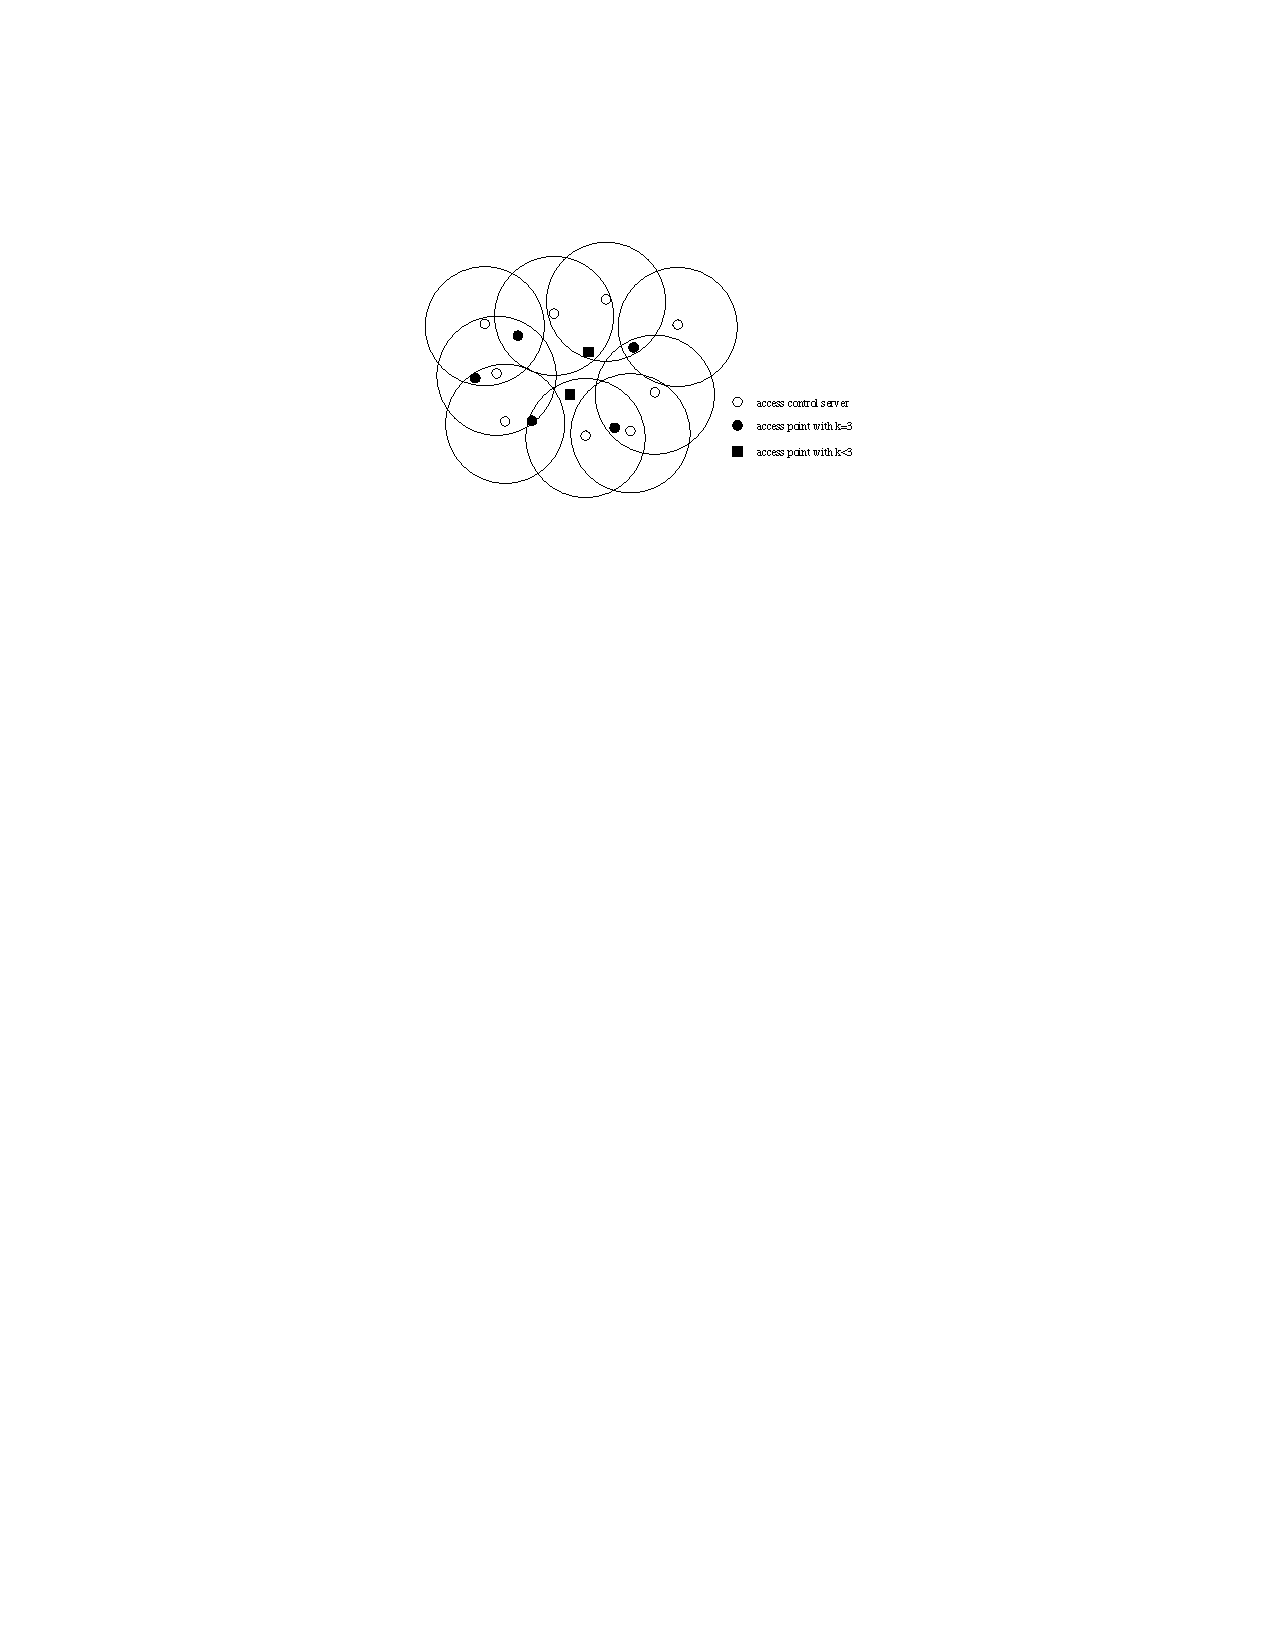
\includegraphics[width=.6\textwidth]{figuras/pervasive_hospital1.pdf}
	\caption{Possível distribuição de pontos de acesso e servidores de controle de acesso em um ambiente médico ubíquo. Círculos pequenos vazados representam servidores de controle de acesso enquanto os círculos maiores representam o alcance de seu sinal. Círculos cheios representam pontos de acesso que ``alcançam'' três servidores, e quadrados cheios representam pontos de acesso que ``alcançam'' menos de três servidores e podem não obter credenciais para acessar o banco.}
	\label{fig:pervasive_hospital1}
\end{figure}

Em um ambiente médico ubíquo, assim como em outros ambientes de computação, é extremamente importante proteger a rede e os computadores do ambiente de uma série de possíveis ataques, como ataques de negação de serviço (\emph{Denial of Service} -- DoS), hackerismos, cavalos de Troia, etc. Serviços de auditoria automática de segurança devem incluir mecanismos básicos~\cite{lunt1988automated,tsudik1990audes}, como detecção de intrusos ou um \emph{firewall}. Em particular, os mecanismos devem ser aprimorados para proteger uma infraestrutura altamente \textbf{heterogênea} e \textbf{distribuída}, como um sistema ubíquo. Por exemplo, um sistema distribuído de detecção de intrusos como proposto em~\cite{bass2000intrusion} consegue lidar com diversos tipos de ataques distribuídos. O próprio serviço de auditoria deve possuir suporte de tolerância a falhas, o que inclui suporte a operações desconectadas~\cite{kistler1992disconnected} para manter o serviço em desconexões transientes. Por exemplo, sensores distribuídos podem ter que \emph{bufferizar} dados durante o período de desconexão da rede.

Além destes fatores, decisões de arquitetura devem ser tomadas de forma aumentar, robutez, escalabilidade e autonomia do sistema médico ubíquo. A ideia é permitir que o sistema seja adaptativo de tal forma que diferentes regiões físicas do sistema funcionem de maneira independente. Por exemplo, um incêncio em uma ala de um hospital, resultando em perdas de pontos e servidores de acesso ubíquo, não deve fazer com que o sistema inteiro interrompa os serviços. Além disso, expandir o sistema deve ser uma tarefa simples.

% subsection questões_de_medicina (end)

Soluções desenvolvidos em outras sub-áreas da computação podem ser interessantes para a computação ubíqua, por exemplo, em~\cite{parikhformally} o autor apresenta um protótipo de arquitetura many-core com NoC (\emph{Network on Chip}) e roteadores autorreconfiguráveis e tolerantes a falhas em nível de \emph{hardware}.
